\raggedright

To this day, there have been many proposals and solutions to mitigate the \textit{effects} of a DDoS attack, however there are no methods to protect against all forms of DDoS attacks.
This is because that new types of attacks are continually being developed to bypass the constant countermeasures employed by victims.

\vspace{0.5cm}

\begin{figure}[h]
	\centering
	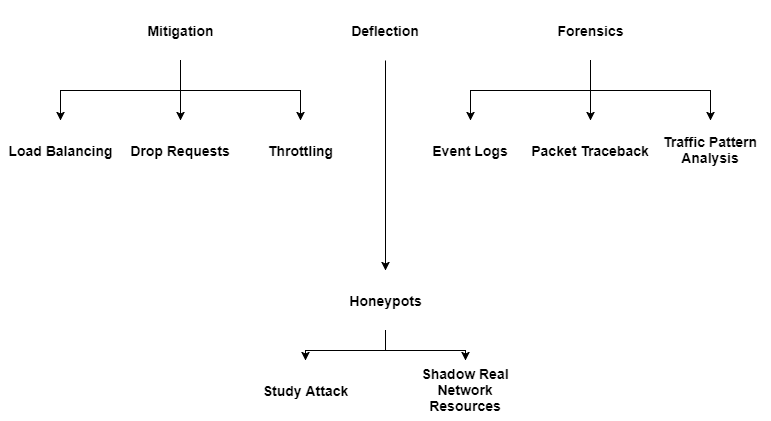
\includegraphics[width=0.75\linewidth]{img/ddos_prevention_tree.png}
	\caption{Countermeasures Employed Against DDoS Attacks\textsuperscript{\cite{specht2003taxonomies}}}
\end{figure}

\vspace{0.5cm}

The tree above shows three main categories of preventing and mitigating a DDoS attack, as well as examples of procedures in each category. These however are not the only countermeasures employed, as described above there are no methods to protect against all forms of DDoS attacks due to the continuous development and advancement of attack vectors.